\chapter{Electromagnetic Waves}

\textit{When I talk about the fields swishing through space, I have a terrible confusion between the symbols I use to describe the objects and the objects themselves.}\\
\noindent\textbf{-   Richard Feynmann}

\vspace{1cm}

\begin{marginfigure}%
  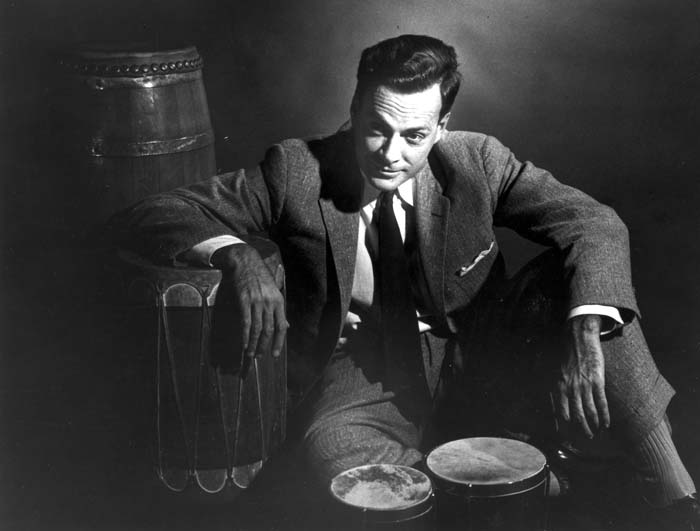
\includegraphics[width=\linewidth]{feynman.jpg}
  \caption{Richard Feynman with his bongos}
  \label{fig:marginfig}
\end{marginfigure}

\noindent Electromagnetic waves are synchronized oscillations of electric and magnetic fields.   They propagate at the speed of light through a vacuum.  The oscillations of the two fields are perpendicular to each other and perpendicular to the direction of energy and wave propagation.  The following analysis will derive the existence of electromagnetic waves in empty space.
\marginnote[30pt]{Electromagnetic waves are produced whenever charged particles are accelerated, and these waves can subsequently interact with any charged particles. They carry energy, momentum and angular momentum away from their source particle and can impart those quantities to matter with which they interact. }


\section{Gradient Operator (Grad or Del)}
The gradient operator is a vector whose components evaluate the slope (spatial rate of change) in the x, y and z directions respectively.
$$\nabla=\lim_{\Delta \rightarrow 0}\left[\begin{array}{c} \nicefrac{\Delta }{\Delta x} \\ \nicefrac{\Delta }{\Delta y} \\ \nicefrac{\Delta }{\Delta z}\end{array}\right]=\left[\begin{array}{c} \nicefrac{d }{d x} \\ \nicefrac{d }{d y} \\ \nicefrac{d}{d z}\end{array}\right]$$


\section{Divergence Theorem (Div)}
The divergence is the gradient operator dotted into a vector.  A vector field will have a different value for the divergence at every point in space.  The divergence is a scalar quantity representing how much a field emanates from a point in space.  \\
\marginnote[0pt]{$$\nabla \cdot \overrightarrow{E}=\left[\begin{array}{c} \nicefrac{dE_x }{d x} \\ \nicefrac{dE_y }{d y} \\ \nicefrac{dE_z}{d z}\end{array}\right]$$}
The divergence theorem states that the sum of the divergence of a vector field from all points is equal to the flux of the field through the bounding surface.  In other words, the total emanation of a field in a volume of space is equal to the  emanation through the surface of the volume.
$$\oint \overrightarrow{E} \cdot d\overrightarrow{A}=\int \nabla \cdot \overrightarrow{E} \ dV$$

\section{Stoke's Theorem (Curl)}
The curl is the gradient operator crossed into a vector.  A vector field will have a different curl at every point in space.  The curl is a vector quantity representing the circulation occuring at a point in space. 
\marginnote[0pt]{$$\nabla \times \overrightarrow{E}=\left[\begin{array}{c} \nicefrac{dE_z }{d y}-\nicefrac{dE_y }{d z} \\ \nicefrac{dE_x }{d z} -\nicefrac{dE_z }{d x}\\ \nicefrac{dE_y}{d x}-\nicefrac{dE_x }{d y}\end{array}\right]$$}
Stoke's theorem states that the sum of the curl for all points over a surface is equal to the sum of the field directed along the path bounin the surface.  In other words, the total circulation of a field over a surface is equal to the circulation along the perimeter of that area. 
$$\oint \overrightarrow{E} \cdot d\overrightarrow{s}=\int \nabla \times \overrightarrow{E} \cdot d\overrightarrow{A}$$

\section{Maxwell's Equations in Differential Form}
\begin{marginfigure}[100pt]
  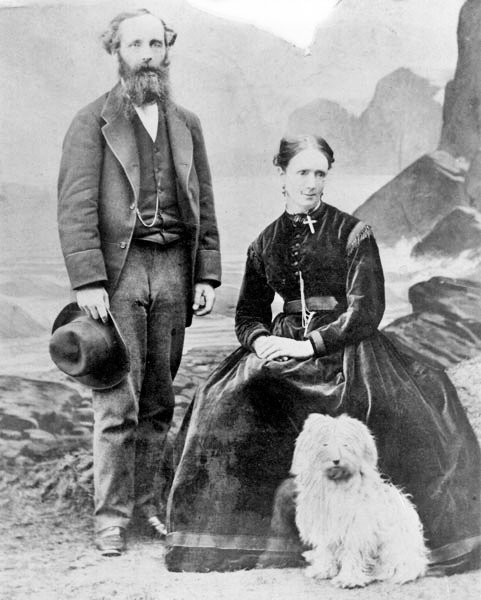
\includegraphics[width=\linewidth]{Maxwell_.jpg}
  \caption{James and Katherine Maxwell with their dog Fluffy McLovely}
  \label{fig:marginfig}
\end{marginfigure}
The mathematical derivation supporting the existence of electromagnetic fields in charge free space begins with expressing Maxwell's equations in differential form.

\subsection{Gauss's Law}
Gauss's law states that the electric flux through the surface of a volume of space is proportional to the amount of charge within that volume.  
$$\oint\overrightarrow{E}\cdot d\overrightarrow{A}=\frac{q_{enc}}{\epsilon_0}$$
By invoking the divergence theorem and expressing the enclosed charge as a integral of the charge density over the volume we can express both side of the equation as volume integrals.
$$ \int \nabla \cdot \overrightarrow{E} \ dV=\int \frac{\rho(\overrightarrow{r})}{\epsilon_0} \ dV$$
Therefore the integrands must be equivalent.
$$\nabla \cdot \overrightarrow{E} =\frac{\rho(\overrightarrow{r})}{\epsilon_0}$$

\subsection{Gauss's Law for Magnetism}
The same approach may be applied to Gauss's law for magnetism.
$$\oint\overrightarrow{B}\cdot d\overrightarrow{A}=0 \hspace{2cm} \oint \nabla \cdot \overrightarrow{B} \ dV=0$$
$$\nabla \cdot \overrightarrow{B} =0$$
Since there is no magnetic charge the right hand side of the equation is zero.  In other words, magnetic fields have zero divergence.  Magnetic fields do not emanate.

\vspace{1cm}
\subsection{Faraday's Law}
Faraday's law explains magnetic induction.  It states that the emf voltage in a loop is equivalent to the time rate of change of the magnetic flux through that loop.  The emf voltage is expressed as the path integral of the electric field around the loop.
$$\oint\overrightarrow{E}\cdot d\overrightarrow{s}=-\frac{d\Phi_B}{dt} $$
The left hand side of the equation may be expressed as an integral over an area using Stoke's theorem.  The right hand side is expressed as an integral over the area by using the definition of magnetic flux.
$$ \int \nabla \times \overrightarrow{E} \cdot d\overrightarrow{A}=-\frac{d}{dt}\int \overrightarrow{B} \cdot d\overrightarrow{A}$$
Once both sides of the equation are expressed as integrals over areas then the integrands may be determined as equal.  Thus we arrive at the differential form of Faraday's law.
$$\nabla \times \overrightarrow{E} =  -\frac{d\overrightarrow{B}}{dt}  $$
The curl off the electric field is equal to the negative of the time rate of change of the magnetic field.

\vspace{1cm}
\subsection{Ampere-Maxwell Law}
Ampere's law states that the line integral of the magnetic field along the boundary of a surface is proportional to the sum of the current and displacement current through a surface bound by said path.  Here the displacement current is the effective current produced by time rate of change of electric field through the surface.
$$\oint\overrightarrow{B}\cdot d\overrightarrow{s}=\mu_0 I+\epsilon_0\mu_0\frac{d\Phi_E}{dt}$$
The left hand side of the equation is transformed into a surface integral of the curl of the magnetic field using Stoke's theorem.  Each term of the right hand side of the equation is also transformed into a surface integral.  The current term is the surface integral of the current density through the surface.  The displacement current term is transformed into the rate of change of the integral of the electric field through the surface.  This second term is further transformed as the surface integral of the time rate of change of the electric field through the surface.
$$ \oint \nabla \times \overrightarrow{B} \cdot d\overrightarrow{A}=\int\mu_0 \overrightarrow{J}\cdot d\overrightarrow{A}+\frac{d}{dt}\int\epsilon_0\mu_0 \overrightarrow{E}\cdot d\overrightarrow{A}$$
Once all terms is the equation are expressed as surface integrals the integrands may be equated to yield the differential form of Ampere's law.
$$\nabla \times \overrightarrow{B} = \mu_0 \overrightarrow{J} +\epsilon_0\mu_0\frac{d\overrightarrow{E}}{dt}  $$

\marginnote[-50pt]{
\noindent \textbf{Maxwell equations differential form:}
$$\nabla \cdot \overrightarrow{E} =\frac{\rho(\overrightarrow{r})}{\epsilon_0}$$
$$\nabla \cdot \overrightarrow{B} =0$$
$$\nabla \times \overrightarrow{E} =  -\frac{d\overrightarrow{B}}{dt}  $$
$$\nabla \times \overrightarrow{B} = \mu_0 \overrightarrow{J} +\epsilon_0\mu_0\frac{d\overrightarrow{E}}{dt}  $$
}
\section{Maxwell's Equations in Charge-Free Space}
Once the differential forms of the Maxwell equations are determined they are considered in charge free space.  In space with no charge the charge density $\rho$, and current density $\overrightarrow{J}$ are both zero.  This yields the four equations shown in the margin.
\marginnote{
\noindent \textbf{Maxwell equations differential form in space without charges:}
$$\nabla \cdot \overrightarrow{E} =0$$ 
$$\nabla \cdot \overrightarrow{B} =0$$
$$\nabla \times \overrightarrow{E} =  -\frac{d\overrightarrow{B}}{dt}  $$
$$ \nabla \times \overrightarrow{B} =\epsilon_0\mu_0\frac{d\overrightarrow{E}}{dt}  $$}
These equations state that the electric and magnetic field have zero divergence in charge free space.  Additionally they state that the curl of the electric field is proportional to the time rate of change of the magnetic field and the curl of the magnetic field is proportional to the time rate of change of the electric field.  Note the high degree of symmetry in this system of equations.\\
To proceed in making sense of these equations we take the third equation and take the curl of both sides.  
$$\nabla \times \left(\nabla \times \overrightarrow{E}\right) = \nabla \times\left( -\frac{d\overrightarrow{B}}{dt}\right)  $$
\marginnote[-50pt]{\subsection{Double Curl}
$$\nabla \times(\nabla \times \overrightarrow{E}) =\nabla (\nabla \cdot  \overrightarrow{E})-\nabla^2\overrightarrow{E}$$
The second term of this identity includes the operator $\nabla^2$.  This is known as the Laplacian operator.  It is a scalar operator.
$$\nabla^2=\nabla \cdot \nabla=\left[\begin{array}{c} \nicefrac{d }{d x} \\ \nicefrac{d }{d y} \\ \nicefrac{d}{d z}\end{array}\right] \cdot \left[\begin{array}{c} \nicefrac{d }{d x} \\ \nicefrac{d }{d y} \\ \nicefrac{d}{d z}\end{array}\right]$$
$$\nabla^2=\frac{d^2 }{d x^2}+\frac{d^2 }{d y^2}+\frac{d^2 }{d z^2}$$}
On the left hand side of the equation we confront the double curl.  The double curl is the curl of the curl.  Whoa.  Using the identity detailed in the margin the left hand side of the equation becomes tractable.  On the right hand side of the equation the order of applying the the curl and time derivative are reversed.
$$\nabla (\nabla \cdot  \overrightarrow{E})-\nabla^2\overrightarrow{E}= -\frac{d \left( \nabla \times\overrightarrow{B}\right) }{dt} $$
At this point things simplify greatly.  The first term on the left hand side of the equation is zero since the electric field has no divergence in charge free space.  The right hand side of the equation which includes the curl of the magnetic field may make use of the last of Maxwell's equations. 
$$-\nabla^2\overrightarrow{E}= -\frac{d \left( \epsilon_0\mu_0\frac{d\overrightarrow{E}}{dt}\right) }{dt}  $$
Finally the analysis arrives at the following equation which states that the spatial curvature of the field is proportional to 
$$\nabla^2\overrightarrow{E}= \epsilon_0\mu_0\frac{d^2 \overrightarrow{E} }{dt^2}  $$


\section{Wave Equations}
\marginnote[0pt]{\subsection{Scalar Wave Equation}
$$\nabla^2 u=\frac{1}{v^2}{\partial^2 u \over \partial t^2} $$
Solutions to the scalar wave equation are sinusoidal scalar waves with wave speed $v$.}
Performing a near identical set of operations on the magnetic field yields an equivalent equation for the magnetic field.  The two equations are listed below.
$$\nabla^2\overrightarrow{E}=\epsilon_0\mu_0\frac{d^2\overrightarrow{E}}{dt^2} $$
$$\nabla^2\overrightarrow{B}=\epsilon_0\mu_0\frac{d^2\overrightarrow{B}}{dt^2} $$
We recognize these as similar to the scalar wave equation except that they are vectors.

\section{1-D Wave Equation Solutions}
Consider the solution of the one dimensional wave propagating in the positive x-direction.  This is known as a plane wave because the wavefronts cover an infinitely large plane.  Clearly this is an idealization and not physically realizable.  The magnitude of the electric and magnetic components are given below.
$$E=E_{max} \cos(kx-\omega t)$$
$$B=B_{max} \cos(kx-\omega t)$$
The wave speed of the solution is the speed of light, $c$.
$$v=\frac{k}{\omega}=\lambda f=\frac{1}{\sqrt{\epsilon_0\mu_0}}=\frac{E_{max}}{B_{max}}=c$$
$$c=3.00\times 10^8 \frac{\text{meter}}{\text{second}}$$

\section{Poynting Vector}
The Poynting vector represents the rate of energy flow through a unit surface area perpendicular to the direction of wave propagation.  The Poynting vector points in the same direction that the wave propagates.


\begin{minipage}{7cm}

$$\overrightarrow{S} \equiv \frac{1}{\mu_0} \overrightarrow{E} \times \overrightarrow{B} $$
\end{minipage}
\begin{minipage}{7cm}
\tdplotsetmaincoords{60}{110}
$$\begin{tikzpicture}[scale=1,tdplot_main_coords]
\coordinate (O) at (0,0,0);
\coordinate (P) at (1,2,3);
\draw[very thick,->] (0,0,0) -- (2,0,0) node[anchor=north ]{$B$};
\draw[very thick,->] (0,0,0) -- (0,2,0) node[anchor= west]{$v,S$};
\draw[very thick,->] (0,0,0) -- (0,0,2) node[anchor=south]{$E$};
\end{tikzpicture}
$$
\end{minipage}

\section{Wave Energy}
The intensity of the wave is the power delivered by the wave per unit area.  This is the average value of the Poynting vector.
$$I=S_{av}=\frac{E_{max}B_{max}}{2\mu_0} \hspace{2cm} \frac{E}{B}=c$$
At any instant the energy stored per unit volume is $u$.  The energy per unit volume is split between the electric field and magnetic field evenly.  The electric energy per unit volume and magnetic energy per unit volume are $u_E$ and $u_B$ respectively.
$$u_E=\frac{\epsilon_0}{2}E^2 \hspace{2cm} u_B=\frac{1}{2\mu_0}B^2 \hspace{2cm} u_E=u_B$$
The time average energy per unit volume is half the total maximum energy per unit volume.
$$u=u_E+u_B \hspace{2cm} u_{av}=\frac{u_{max}}{2}$$
The intensity is the product of the speed of light and the average energy per unit volume.
$$I=S_{av}=cu_{av}$$

\section{Momentum and Radiation Pressure}
Electromagnetic radiation carries a volumetric momentum density and applies a radiation pressure when it impacts a surface.
\subsection{Complete Absorption}
When hitting a radiation absorber the impulse $\Delta p$to the surface is the wave energy, $U$, divided by its velocity, $c$.  The radiation pressure $P$ is the intensity divided by its speed.
$$\Delta p=\frac{U}{c} \hspace{2cm} P=\frac{S}{c}$$
\subsection{Complete Reflection}
In the case of a reflector the impulse and pressure are double.
$$\Delta p=\frac{2U}{c} \hspace{2cm} P=\frac{2S}{c}$$

\section{Polarization (Malus's Law)}
Light may have electric fields in any direction perpendicular to its direction of propagation.  Polarized light is light that has all of its electric field aligned in a single direction.  Filters may be used to align the polarization along a particular direction.
\subsection{Polarized Light}
When polarized light passed through a polarizing filter the intensity of the transmitted light is as follows.
$$I_{transmitted}=I_0\cos^2 \theta$$
\subsection{Unpolarized Light}
For unpolarized light traveling through a polarizing filter the following behavior is observed.
$$I_{transmitted}=\frac{I_0}{2}$$

\section{Spectrum of Electromagnetic Waves}
In free space the frequency of electromagnetic radiation completely determines its wavelength since the speed of light is constant.
$$c=f \lambda$$
Below is a diagram detailing various wavelengths of electromagnetic radiation.
\begin{center}
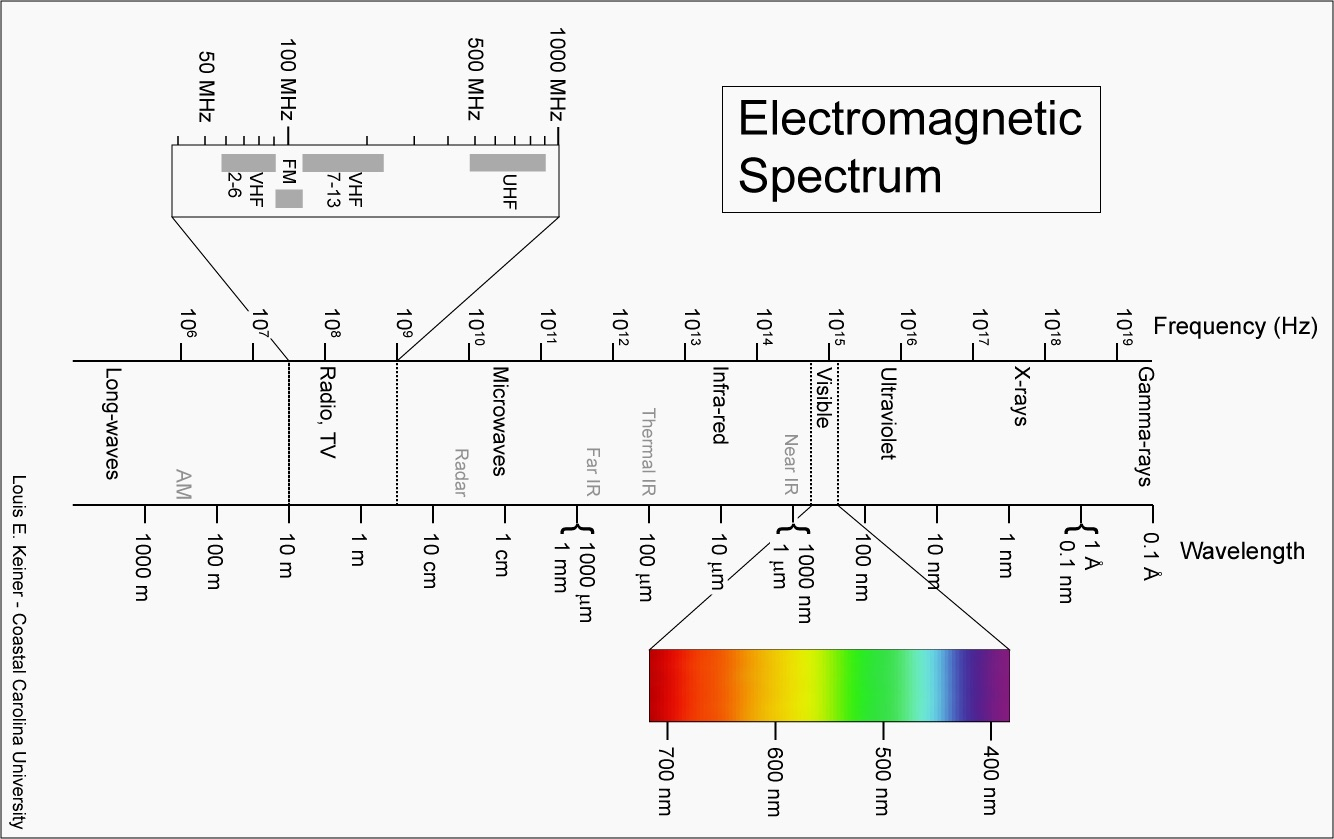
\includegraphics[height=4in,width=6in,angle=0]{spectrum.jpg}

\end{center}
